% --- tv1_duc.tex ---
% Phân tích Nhóm 1: Xu hướng Doanh thu theo Thời gian
\newpage
\vspace{0.6cm}
\noindent\textbf{3. Kết quả phân tích \& Trực quan hóa:}

% (a) Biến động theo tháng/quý
\begin{enumerate}[label=(\alph*)]
    \item \textbf{Biến động theo tháng/quý:}
\end{enumerate}

\begin{figure}[H]
    \centering
    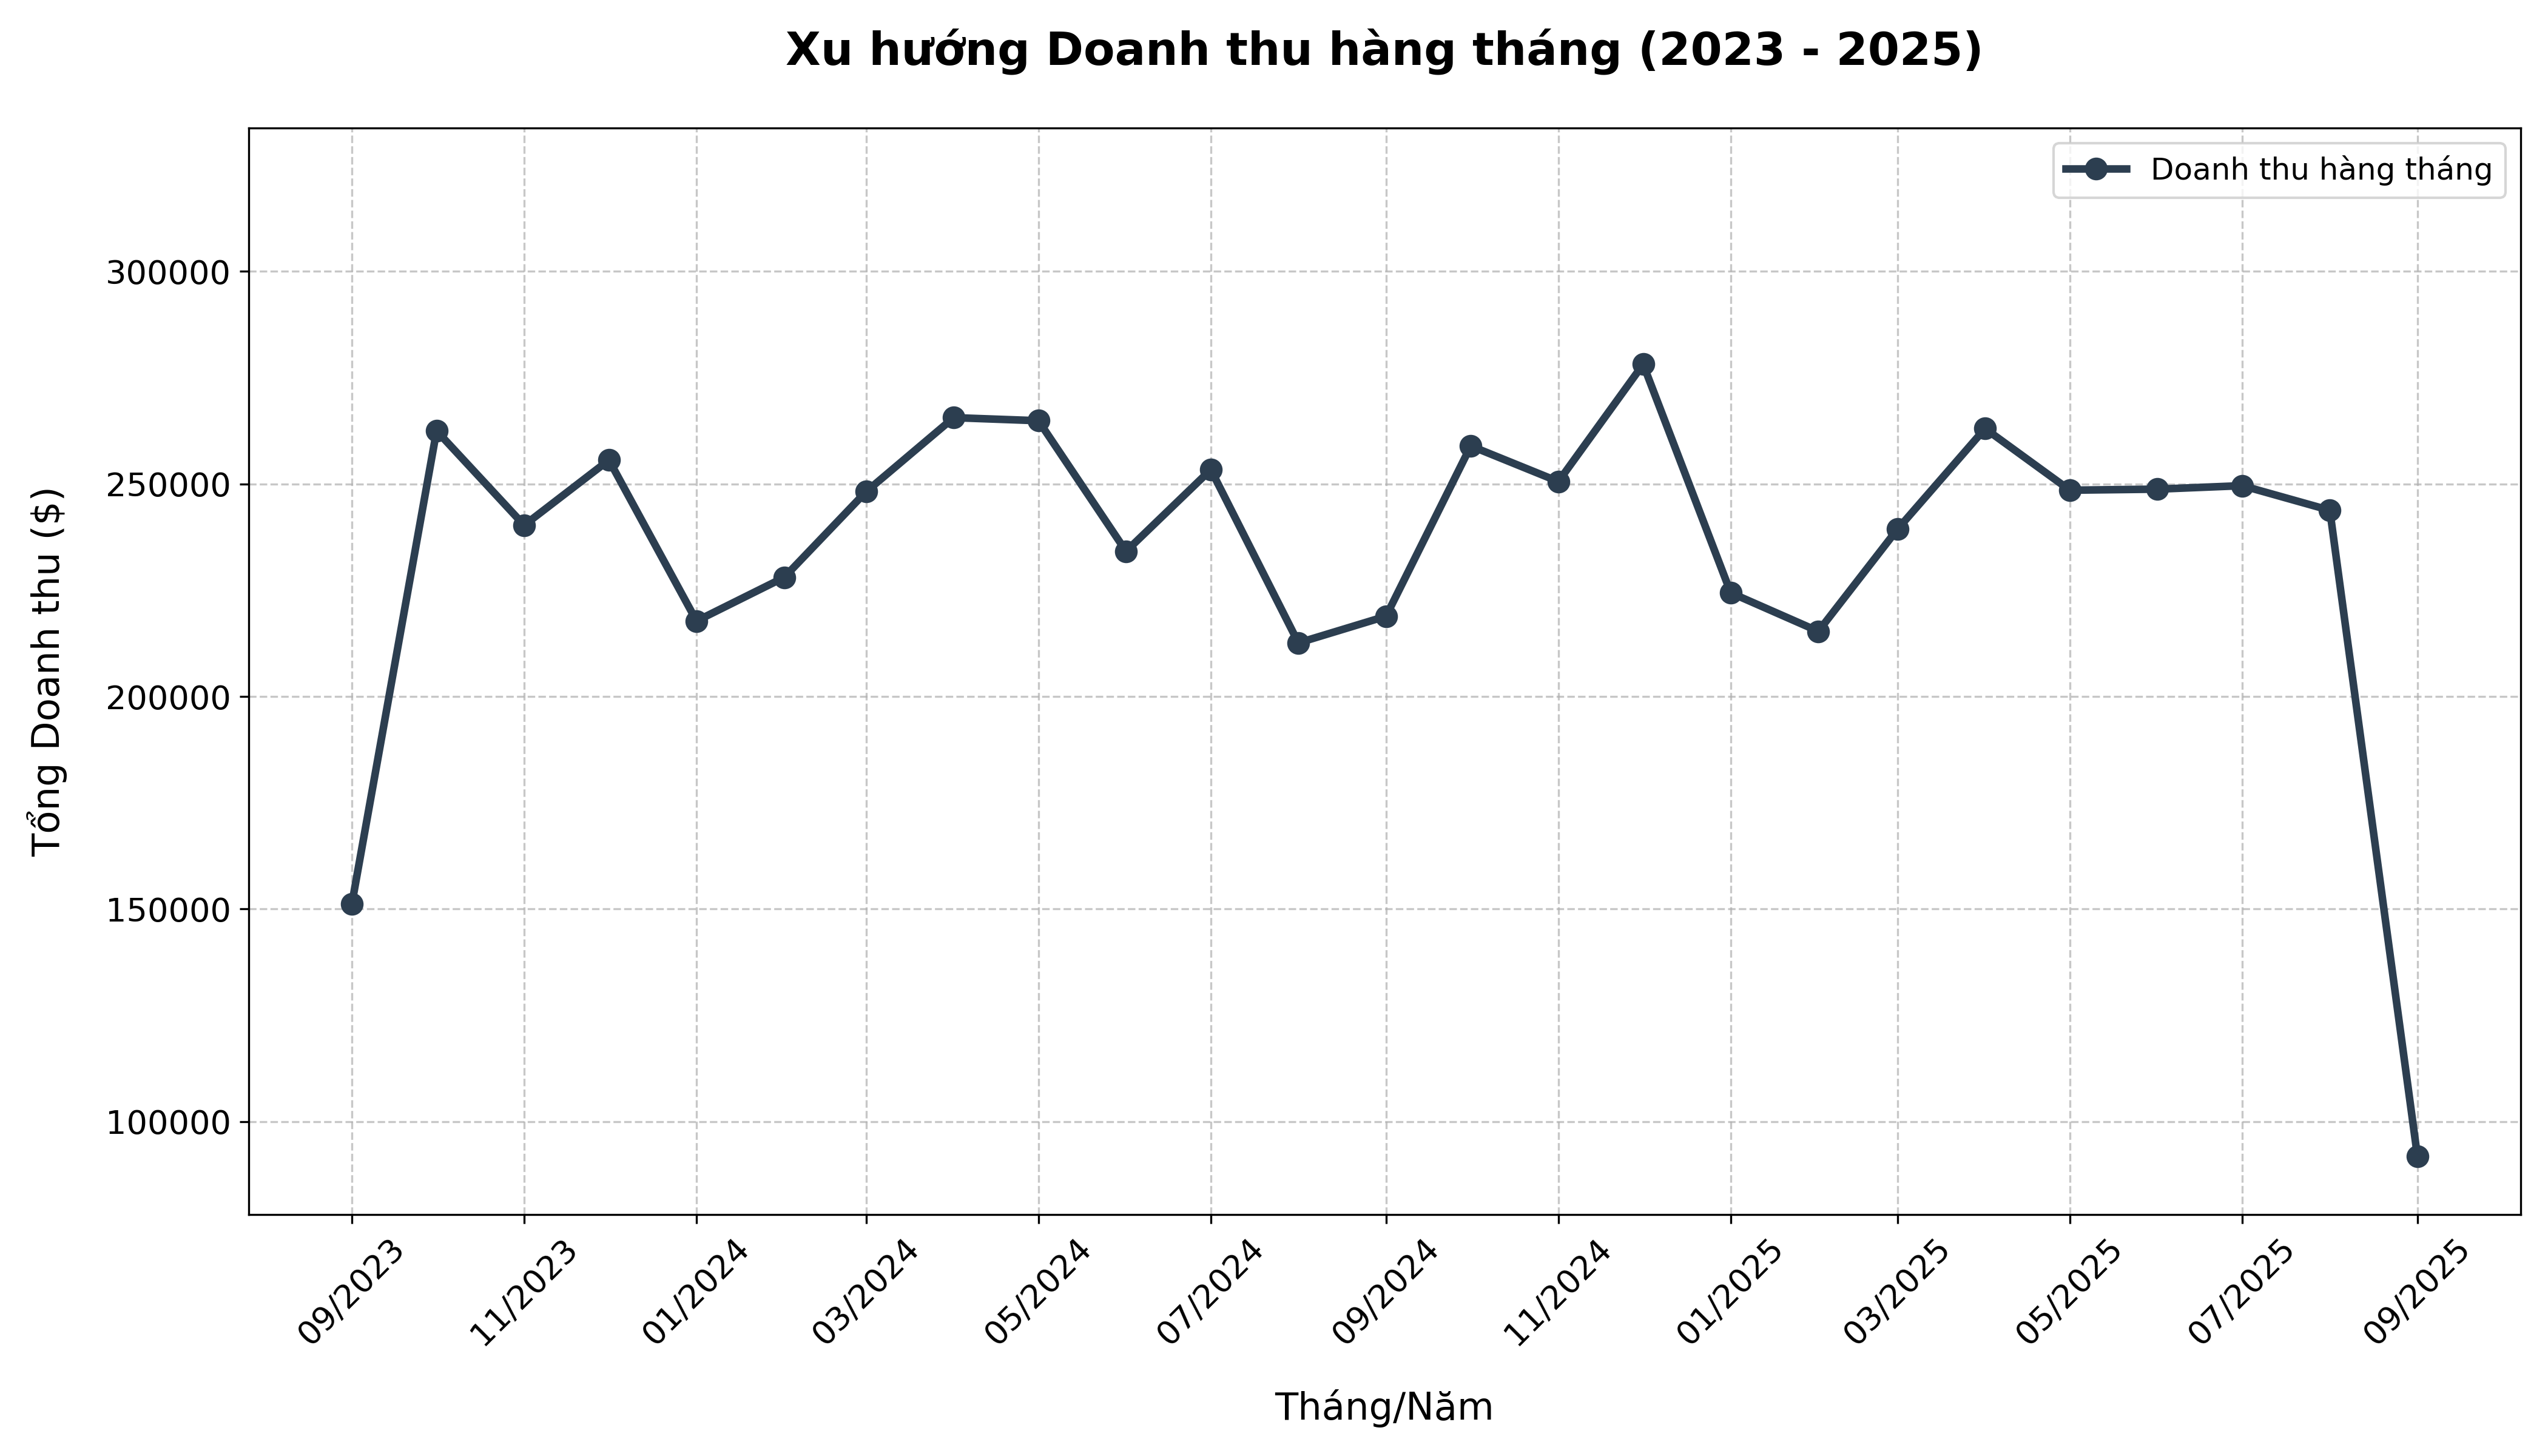
\includegraphics[width=1\textwidth]{images/revenue_trend.png}
    \caption{Biểu đồ xu hướng doanh thu hàng tháng từ 2023 - 2025}
    \label{fig:revenue_trend}
\end{figure}

\begin{itemize}
    \item \textbf{Biến động theo Tháng (Monthly Trend):}
    \begin{itemize}[label=--]
        \item \textit{Xu hướng tổng thể:} Doanh thu duy trì ở mức ổn định nhưng có xu hướng biến động mạnh theo từng tháng. Đặc biệt, điểm thấp nhất toàn kỳ rơi vào \textbf{tháng 9/2025}, đánh dấu sự sụt giảm đáng kể so với các giai đoạn trước đó.
        \item \textit{Các đợt biến động:} Ghi nhận sự tăng trưởng trở lại ngay sau các giai đoạn thấp điểm, cho thấy khả năng phục hồi nhanh của thị trường.
    \end{itemize}
\end{itemize}

\begin{figure}[H]
    \centering
    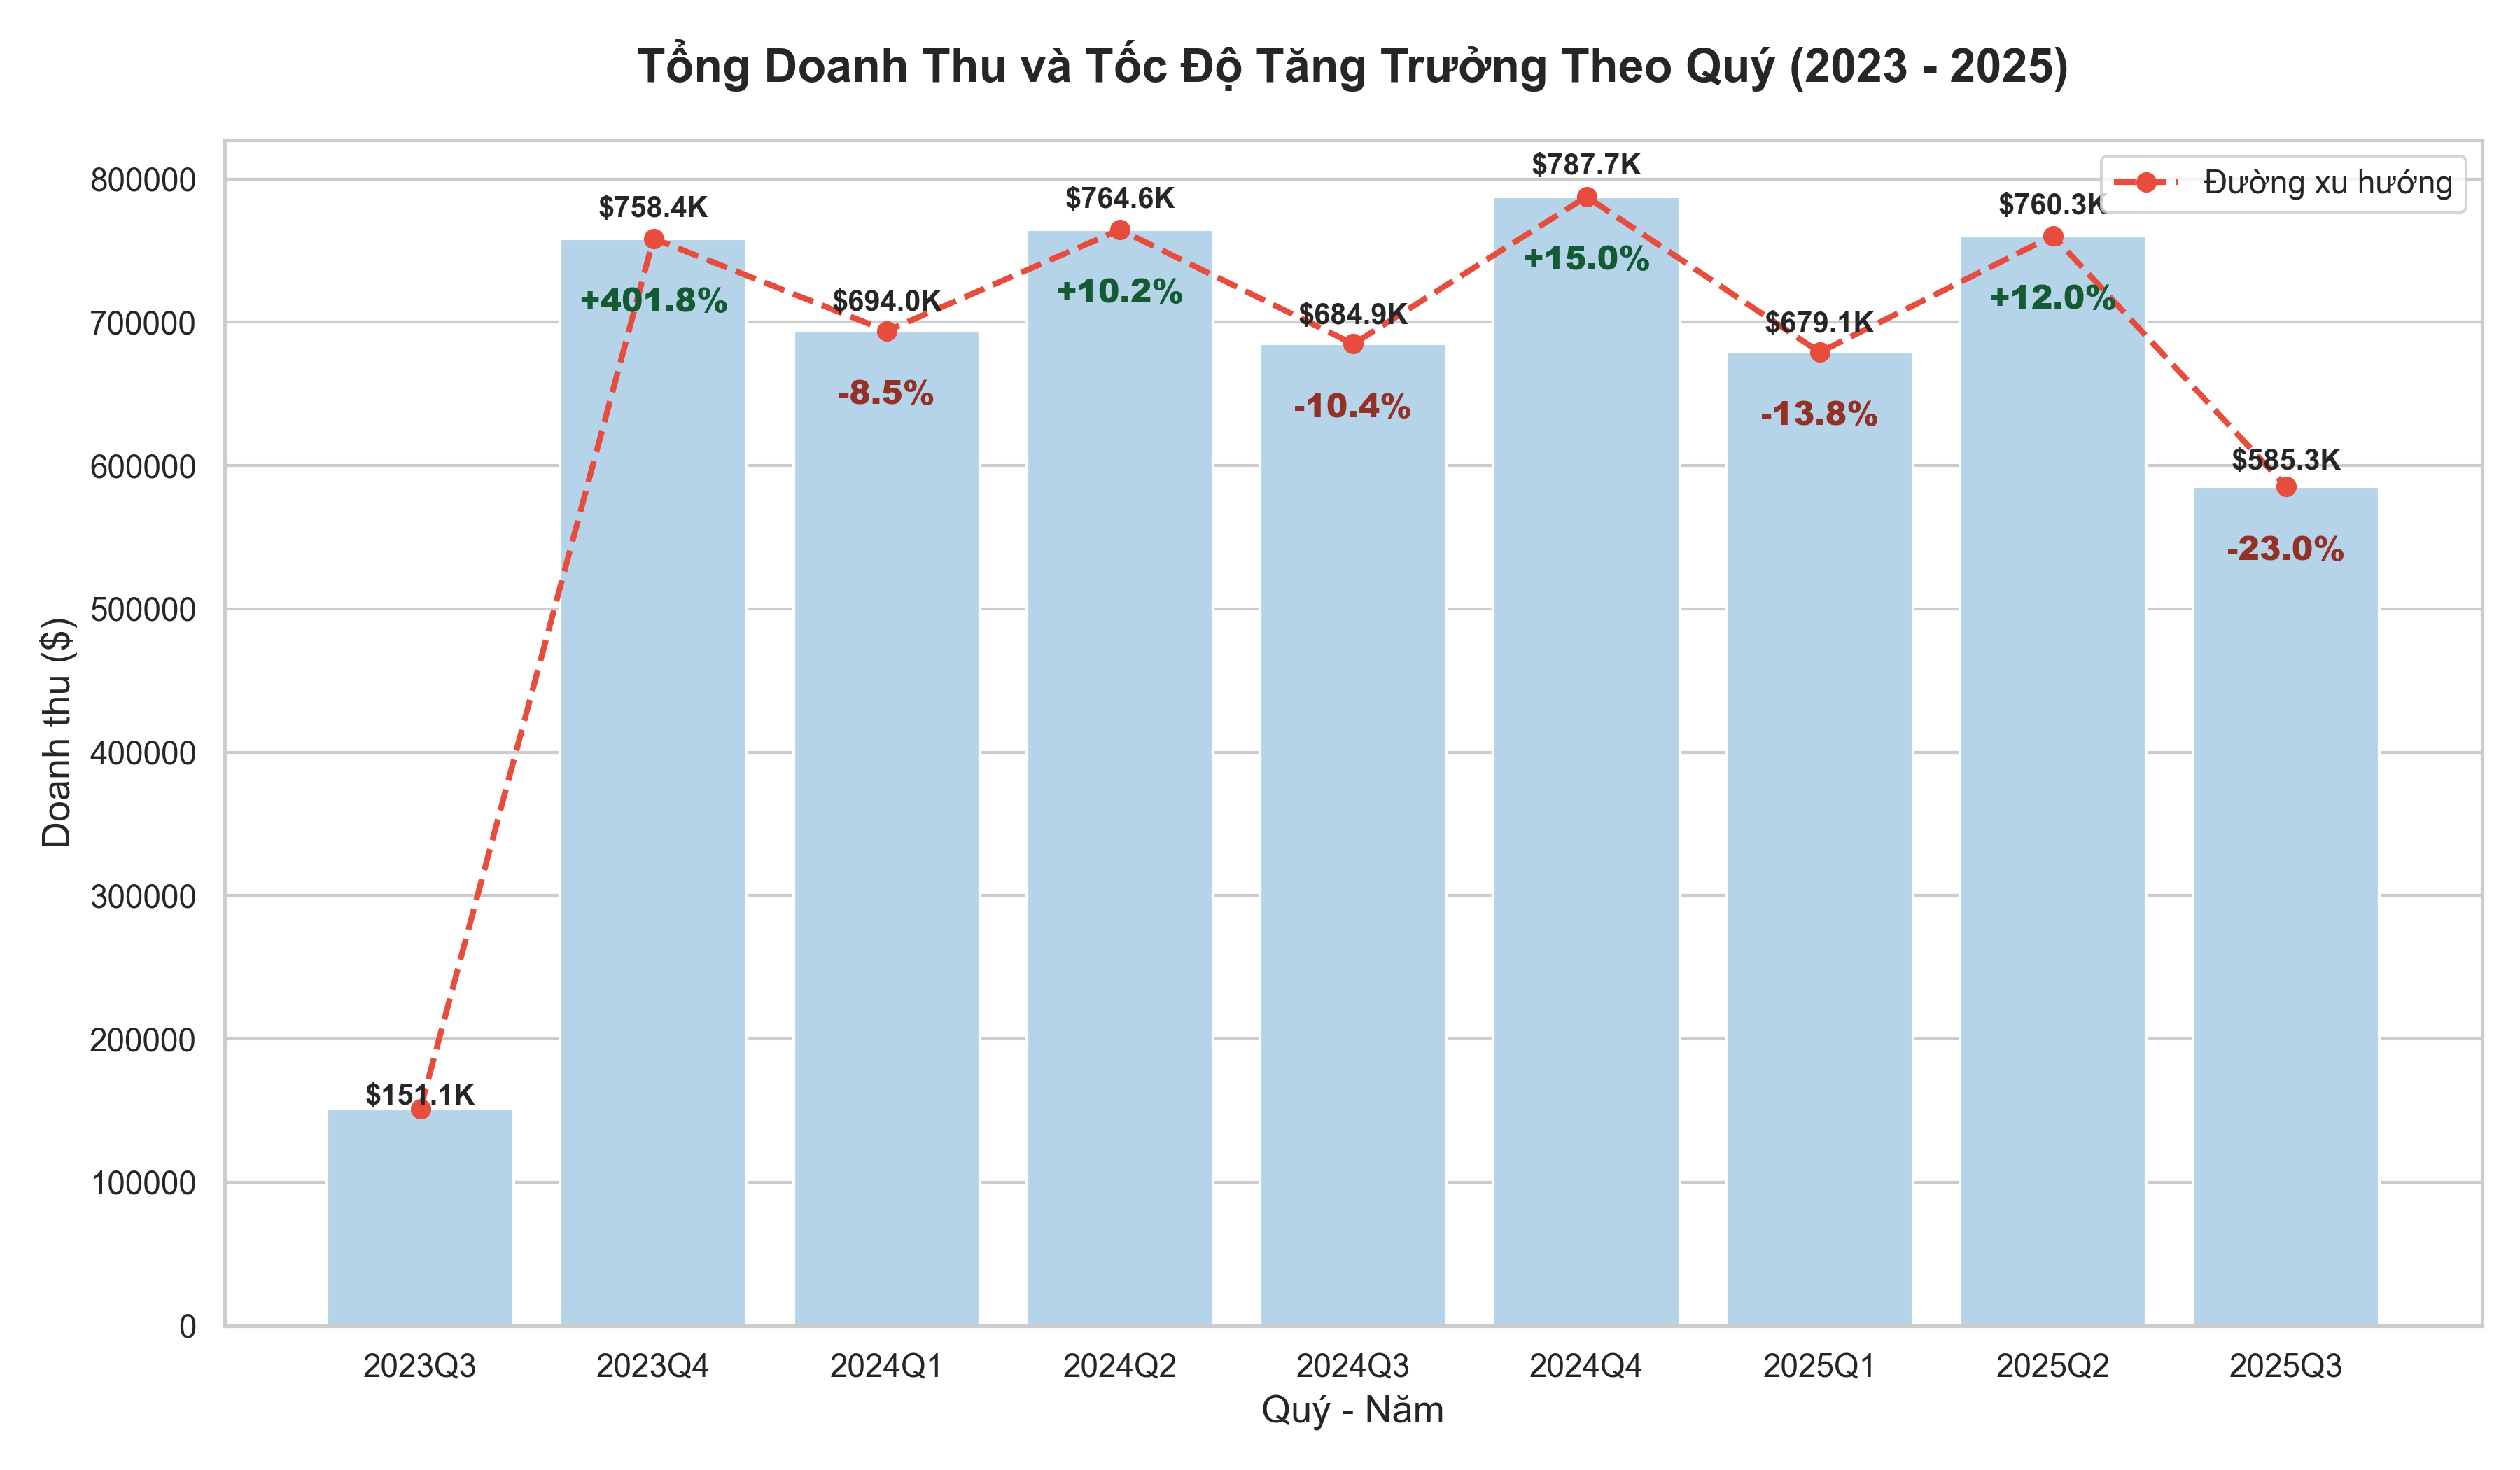
\includegraphics[width=1\textwidth]{images/quarterly_revenue.png}
    \caption{Biểu đồ tổng doanh thu và tốc độ tăng trưởng theo quý}
    \label{fig:quarterly_revenue}
\end{figure}

\begin{itemize}
    \item \textbf{Biến động và Tăng trưởng theo Quý (Quarterly Growth):}
    \begin{itemize}[label=--]
        \item \textit{Tăng trưởng 2024:} Năm 2024 ghi nhận sự bứt phá mạnh mẽ vào \textbf{Quý 2 (+10.2\%)} và đặc biệt là \textbf{Quý 4 (+15.0\%)} - đạt mức doanh thu kỷ lục \$787.7K.
        \item \textit{Các đợt điều chỉnh:} Ngược lại, doanh thu suy giảm vào Quý 1 (-8.5\%) và Quý 3 (-10.4\%), cho thấy tính biến động của thị trường theo từng giai đoạn ngắn hạn trước khi bùng nổ vào cuối năm.
    \end{itemize}
\end{itemize}

% (b) Tháng cao điểm & Mùa vụ
\begin{enumerate}[label=(\alph*), resume]
    \item \textbf{Tháng cao điểm \& Mùa vụ:}
\end{enumerate}

\begin{figure}[H]
    \centering
    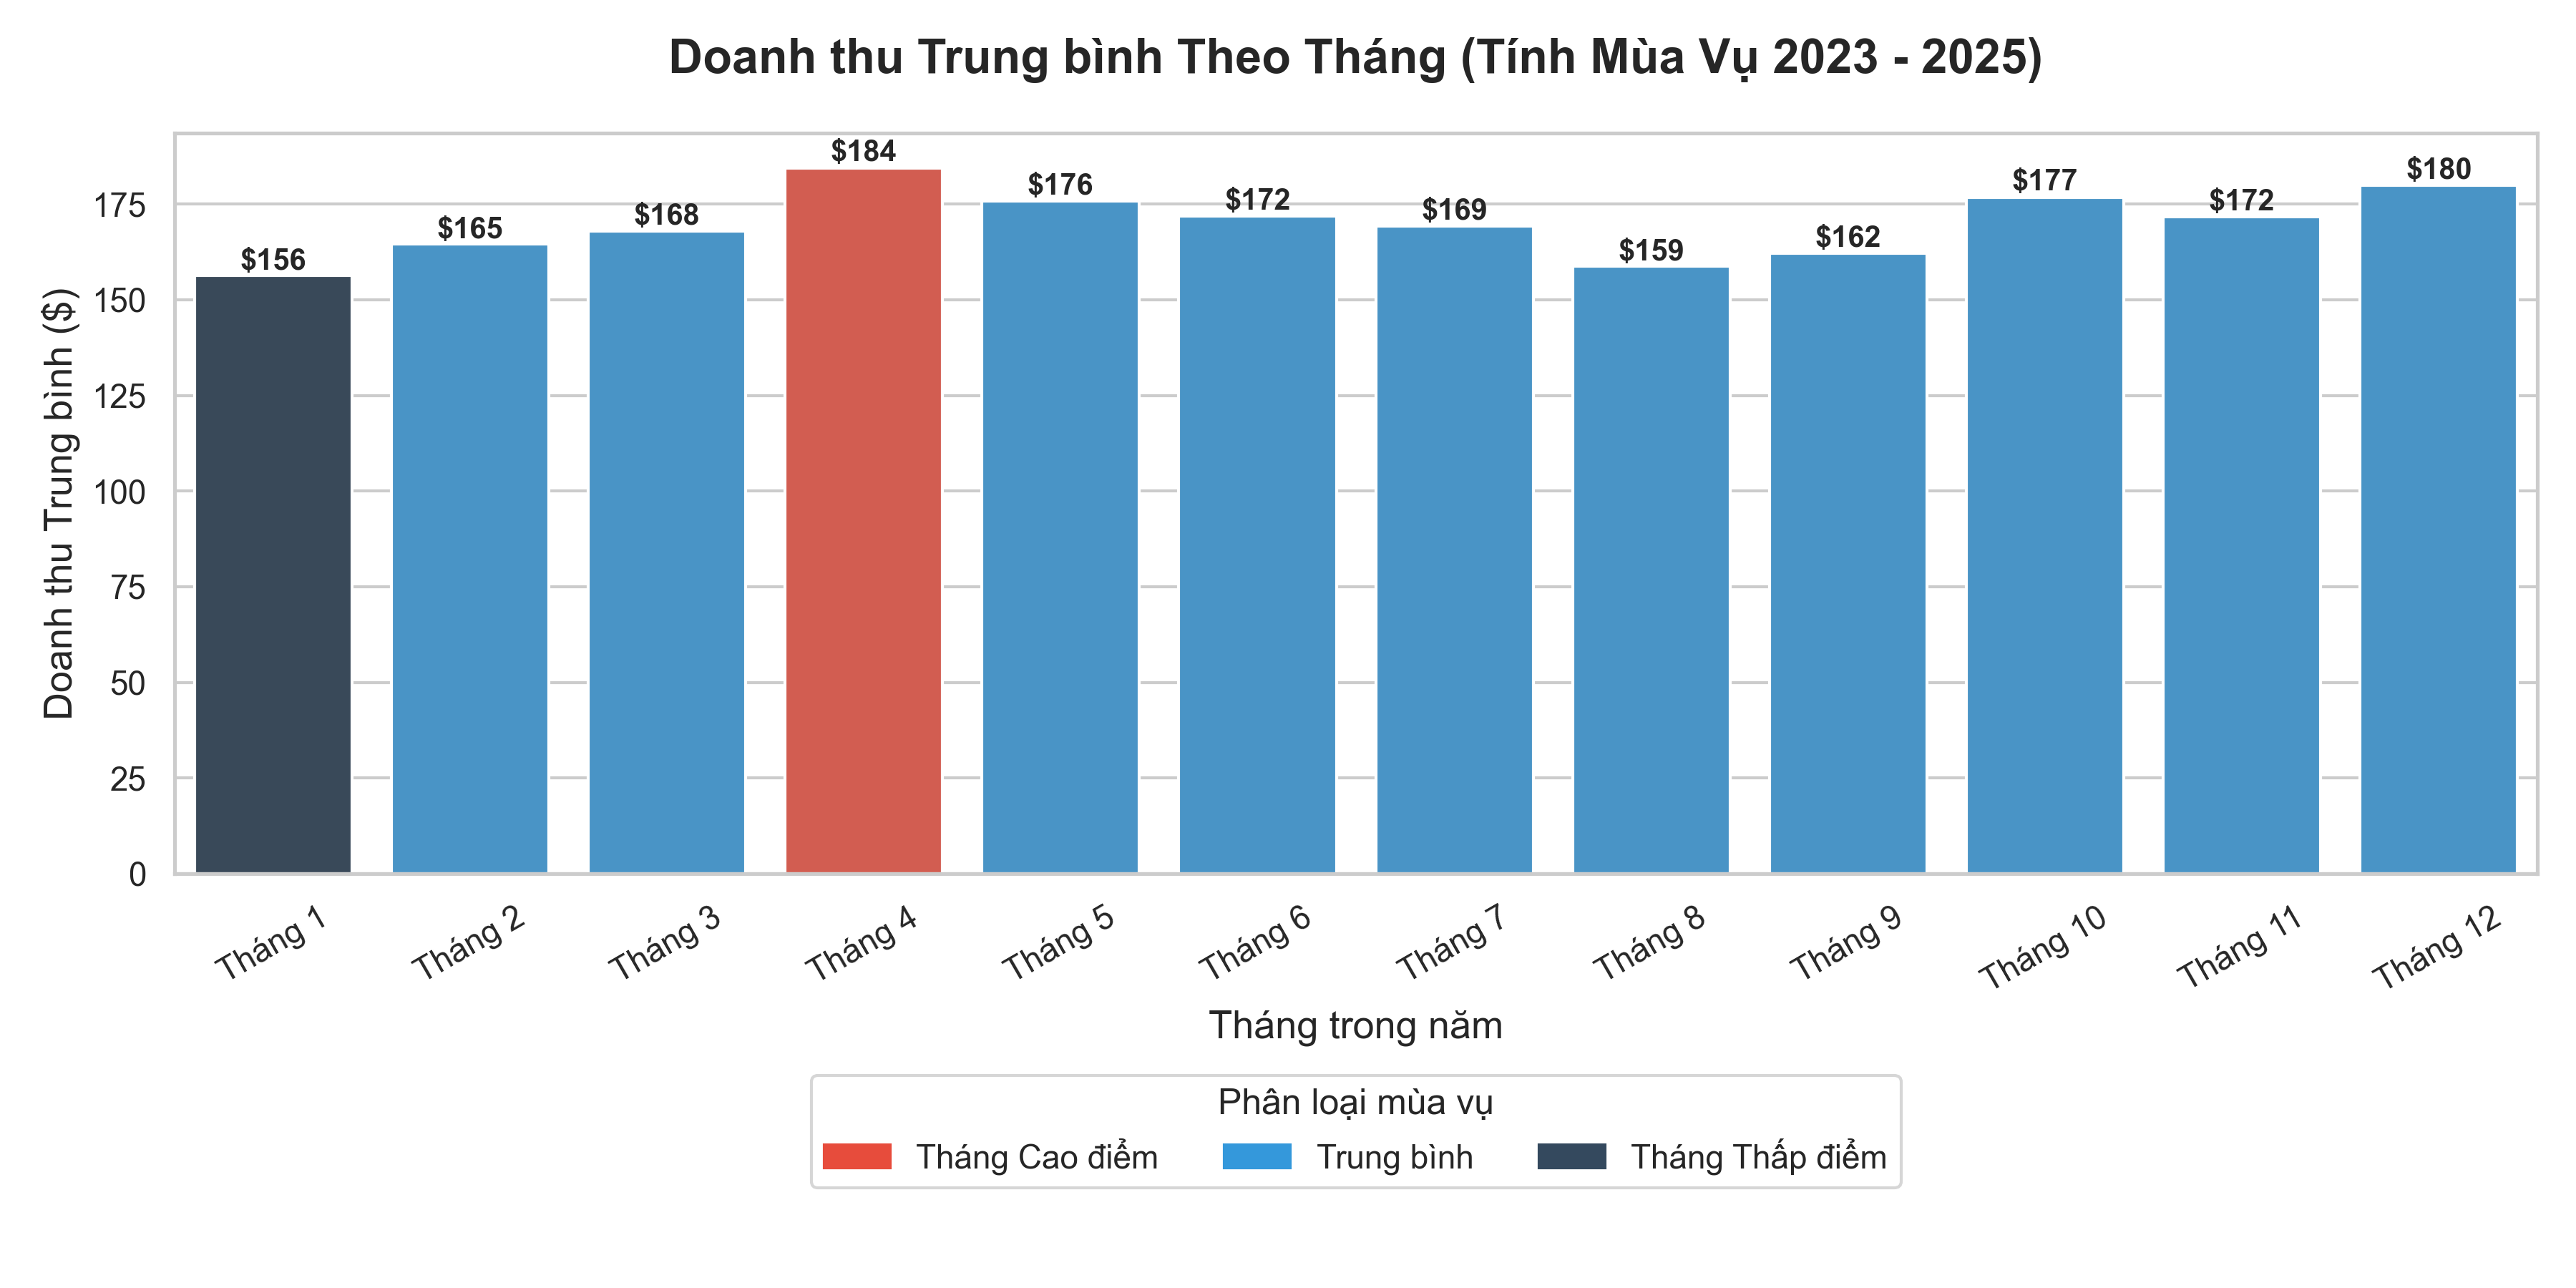
\includegraphics[width=1\textwidth]{images/seasonal_revenue.png}
    \caption{Doanh thu trung bình theo tháng}
    \label{fig:seasonal_revenue}
\end{figure}

\begin{itemize}
    \item \textit{Cao điểm:} Dữ liệu trung bình nhiều năm xác nhận \textbf{Tháng 12 và Tháng 10} là hai tháng mang lại doanh thu cao nhất (trên \$160,000/tháng). Tháng 4 cũng là một điểm sáng mùa vụ quan trọng.
    \item \textit{Thấp điểm:} \textbf{Tháng 1} là tháng có doanh thu trung bình thấp nhất, khớp với biểu đồ mùa vụ (màu xám đậm), phản ánh sự bão hòa chi tiêu sau Tết/Lễ hội.
\end{itemize}

% (c) Xu hướng theo tuần
\begin{enumerate}[label=(\alph*), resume]
    \item \textbf{Xu hướng theo tuần:}
\end{enumerate}

\begin{figure}[H]
    \centering
    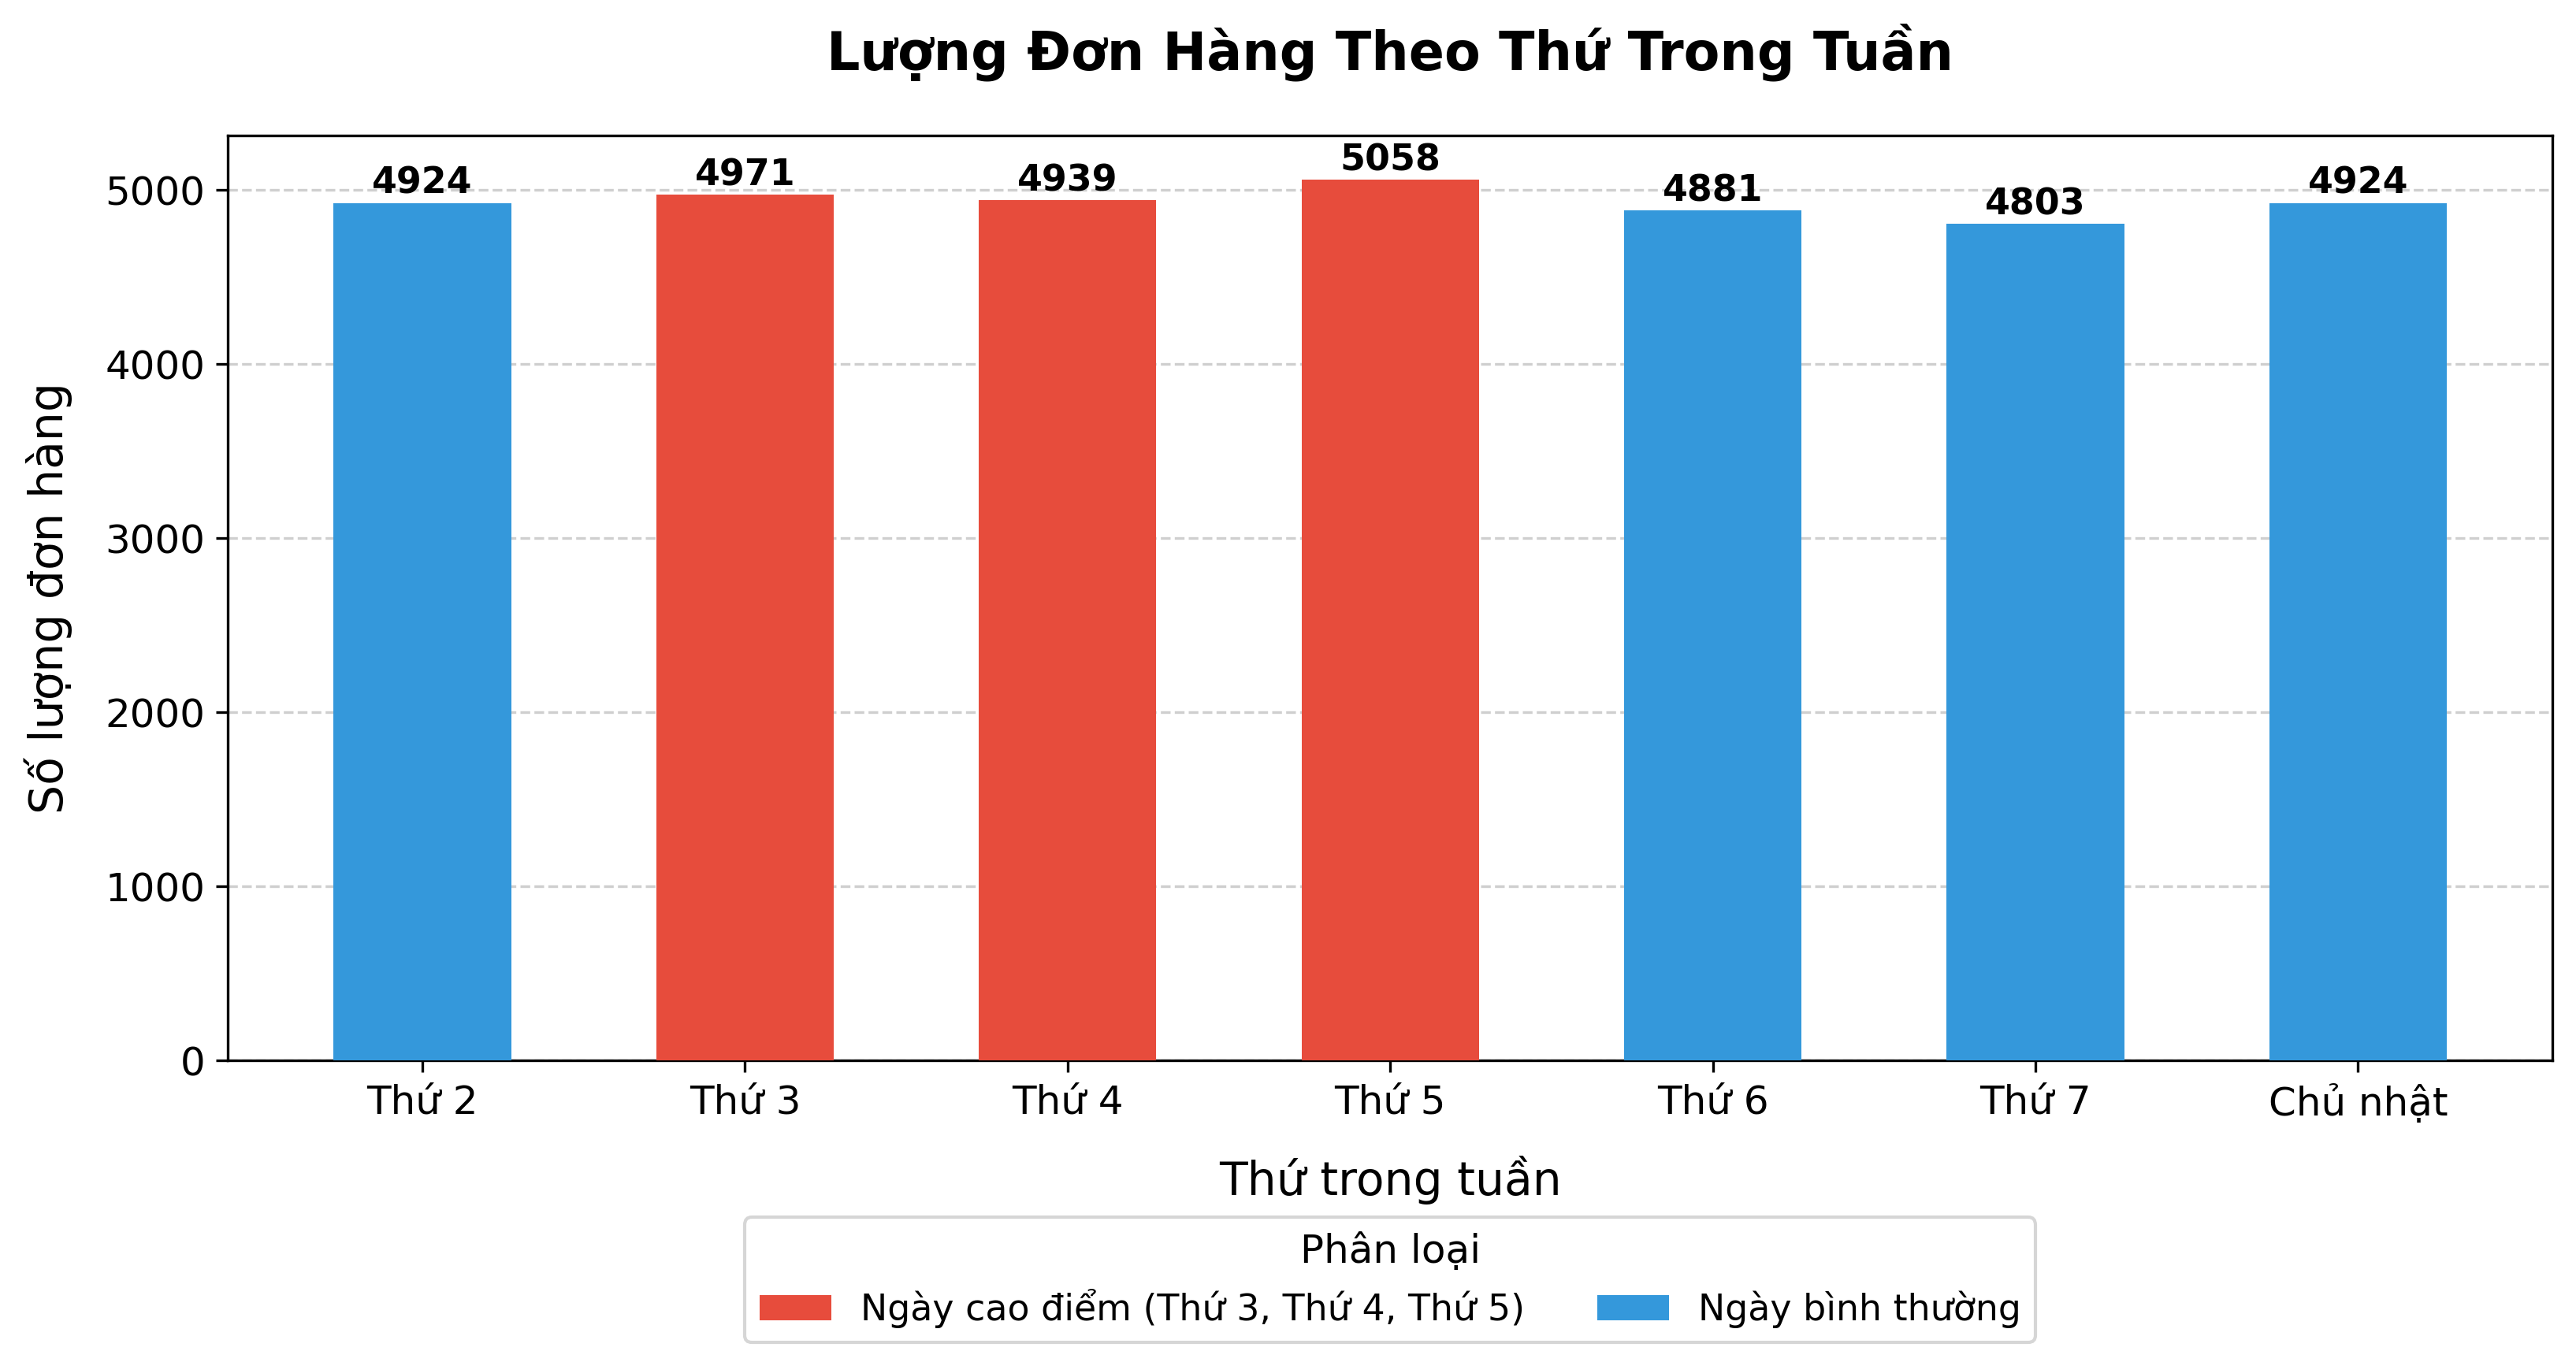
\includegraphics[width=0.88\textwidth]{images/dow_trend.png}
    \caption{Lượng đơn hàng phân bổ theo các thứ trong tuần}
    \label{fig:dow_trend}
\end{figure}

\begin{itemize}
    \item Nhìn vào biểu đồ cột, có thể thấy rõ \textbf{Thứ Ba, Thứ Tư và Thứ Năm} là các ngày cao điểm nhất trong tuần (trong đó Thứ Năm vượt mốc 5,000 đơn hàng). Lượng giao dịch tập trung cực lớn vào giai đoạn giữa tuần, trong khi các ngày cuối tuần (Thứ Bảy, Chủ Nhật) lại có lượng giao dịch thấp hơn. Điều này cho thấy thói quen mua sắm trực tuyến gắn liền với thời gian làm việc hành chính của khách hàng.
\end{itemize}

\vspace{0.3cm}
\noindent\textbf{4. Đưa ra quyết định trong tương lai:}
\begin{itemize}
    \item \textbf{Quản lý kho vận (Inventory):} Tăng cường dự trữ hàng hóa từ tháng 9 để chuẩn bị cho cao điểm quý IV. Đặc biệt chú trọng các mặt hàng chủ chốt vào tháng 4.
    \item \textbf{Chiến lược Marketing:} Đẩy mạnh các chương trình khuyến mãi vào giai đoạn đầu năm (tháng 1 và tháng 2) để kích cầu trong thời kỳ thấp điểm.
    \item \textbf{Tối ưu hóa nhân sự:} Phân bổ thêm nhân lực xử lý đơn hàng vào các ngày giữa tuần để đảm bảo thời gian giao hàng nhanh nhất.
\end{itemize}